
\section{Seikkailijoiden sivut}\label{sec:seikkailijat}


\vspace*{-0.32cm}
\begin{multicols}{2}
\noindent \textbf{Vitsi kulma!\\}
\bigskip
Mä meen ostaan Teslan\\
Tesla: ääh!\\
\bigskip
Voi vitsit! Täällä sataa lunta!\\
Lumi: Täh? En mä sada.

\vfill
\noindent Elna

\columnbreak
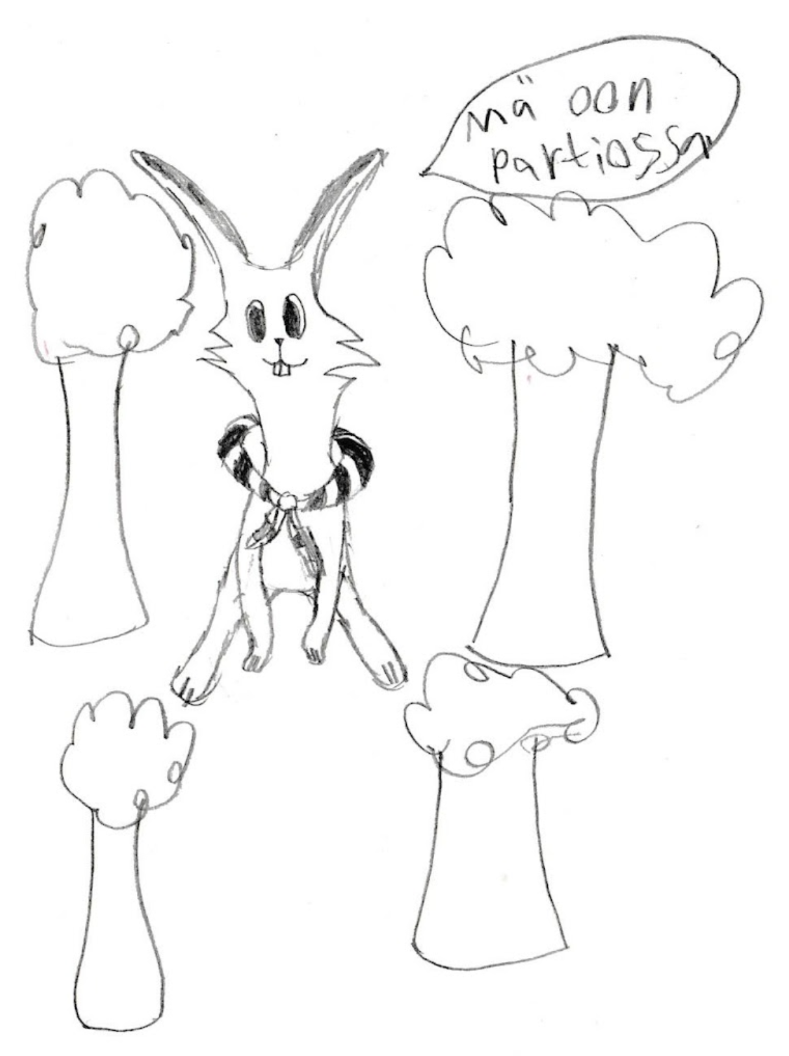
\includegraphics[width=0.42\textwidth]{assets/seikkailijat2}
\end{multicols}

\hrule

\begin{multicols}{2}
\noindent\textbf{Partion ristikko}
\begin{enumerate}
	\item Missä me ollaan
	\item Latinaksi se on Lepus Europaeus
	\item Puinen muki
	\item Kova ääni joka kuuluu ihmisistä
	\item Pelokkaan vastakohta
\end{enumerate}
\columnbreak
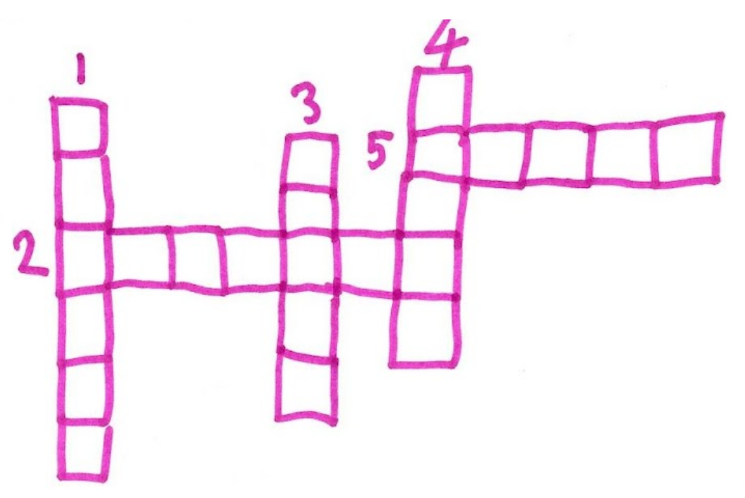
\includegraphics[width=0.5\textwidth]{assets/seikkailijat1}
\end{multicols}


\noindent\textbf{Vitsi aika!}\\
Mitä ruokaa voi syödä kuussa ja maassa? Kuumaa ruokaa!

\bigskip
\noindent\textbf{KYSYMYS!}\\
Jos kyltti kertoo että se on huijaus se tarkoittaa että se on totta, mutta jos se on totta se on totta että se on huijaus.\\
Tätä kutsutaa PARADOXIKSI!

\bigskip
\noindent Kuisma


% \noindent\textbf{Maailman huonoin vitsi!}\\
% Rusakko: No voi vitsit\\
% Puu: Eihän toi ollu vitsi\\
% Ilma: Toi on niin puinen vitsi että puu vastas siihen\\
% Ruoho: Lalala\\
% Lentävä lehmä joka ei näytä lehmältä: Muumaa mums!\\
% Epämuotoinen kukka: Lopeta jo tuolta tulee rusakko\\

% \bigskip
% \noindent Teksti ja kuva: Lillian

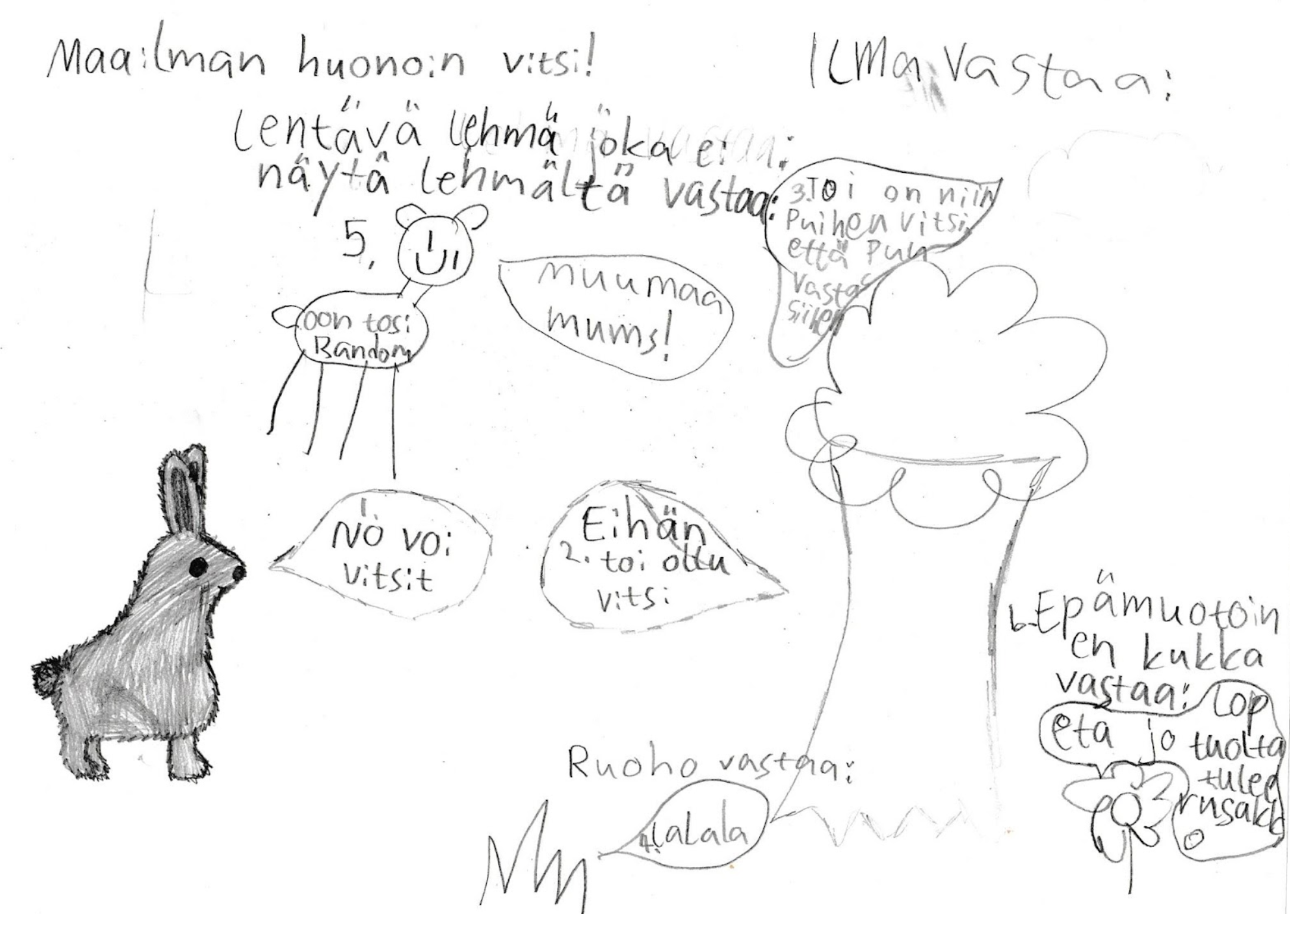
\includegraphics[width=1.0\textwidth]{assets/seikkailijat3}

\bigskip
\noindent Lillian

\bigskip
\hrule

\bigskip
\noindent\textbf{Vitsejä:}\\

\begin{multicols}{2}
\bigskip
\noindent“Mikä on nalle-puhin veli?”\\
“no?”\\
“puh-veli.”\\

\bigskip
\noindent“Kumpi ja Kampi tappelivat.”\\
“Kumpi voitti!”\\

\bigskip
\noindent“miksi darth vader meni \mbox{silmälääkäriin}?”\\
“no?”\\
“hän ei nähnyt Lukea”\\

\columnbreak

\bigskip
\noindent“miksi poliisin ei tarvi käydä \mbox{vessassa}?”\\
“no?”\\
“se pidättää kakkaa.”\\

\bigskip
\noindent“Montako kaksosia on?”\\
“no?”\\
“kaksi”.\\
\end{multicols}


\bigskip
\noindent Samuel


\begin{center}
\noindent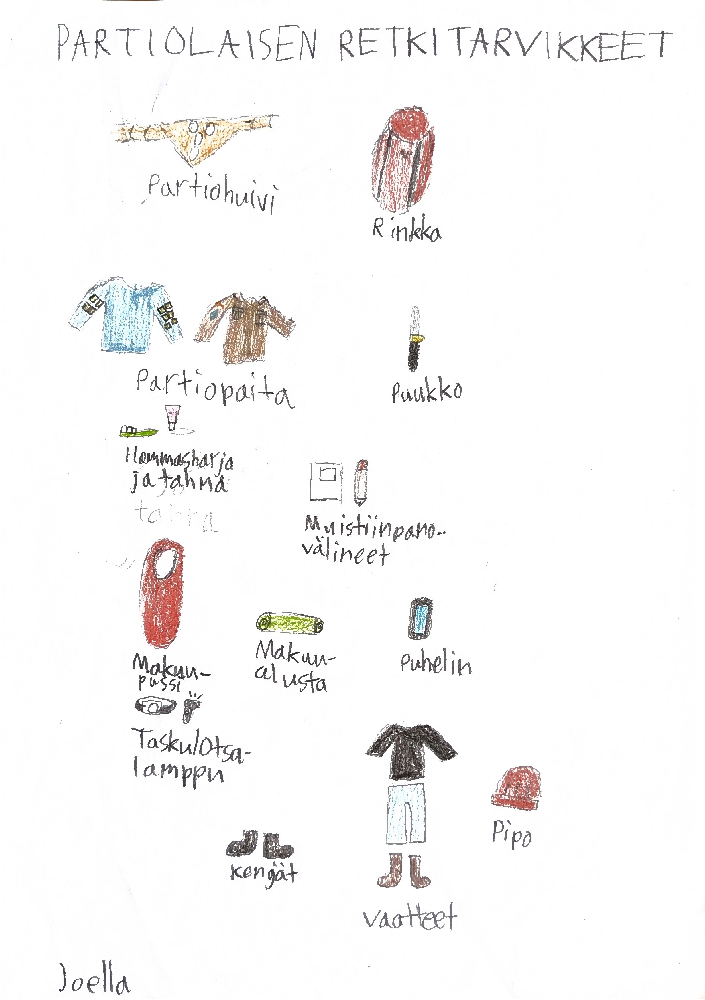
\includegraphics[width=1.0\textwidth,trim={0 0 0 0.5cm},clip]{assets/seikkailijat4}
\end{center}

